\chapter{Output from Dakota}\label{output}

\section{Overview of Output Formats}\label{output:overview}

Given an emphasis on complex numerical simulation codes that run on
massively parallel supercomputers, Dakota's output has been designed
to provide a succinct, text-based reporting of the progress of the
iterations and function evaluations performed by an algorithm. In
addition, Dakota provides a tabular output format that is useful for
data visualization with external tools and a basic graphical output
capability that is useful as a monitoring tool. The JAGUAR Dakota GUI
is an emerging capability that will provide more advanced
visualization facilities in time.

\section{Standard Output}\label{output:standard}

Dakota outputs basic information to ``standard out'' (i.e., the
screen) for each function evaluation, consisting of an evaluation
number, parameter values, execution syntax, the active set vector, and
the response data set. To describe the standard output of Dakota,
optimization of the ``container'' problem (see
Chapter~\ref{additional} for problem formulation) is used as an
example. The input file for this example is shown in
Figure~\ref{output:incont}. In this example, there is one equality
constraint, and Dakota's finite difference algorithm is used to
provide central difference numerical gradients to the NPSOL optimizer.
\begin{figure}
  \begin{small}
    \begin{bigbox}
      \verbatimtabinput[8]{container_opt_npsol.in}
    \end{bigbox}
  \end{small}
  \caption{Dakota input file for the ``container'' test problem --
see \texttt{Dakota/examples/users/container\_opt\_npsol.in} }
  \label{output:incont}
\end{figure}

\clearpage

A partial listing of the Dakota output for the container optimization
example follows:
\begin{small}
\begin{verbatim}
Running MPI executable in serial mode.
Dakota version 5.0 released 12/21/2009.
Subversion revision 5635M built Dec 18 2009 17:19:56.
Constructing Single Method Strategy...
Writing new restart file dakota.rst
methodName = npsol_sqp
gradientType = numerical
Numerical gradients using central differences
to be calculated by the dakota finite difference routine.
hessianType = none

>>>>> Running Single Method Strategy.

>>>>> Running npsol_sqp iterator.





                     NPSOL  ---  Version 5.0-2      Sept 1995
                     ========================================

------------------------------------------
Begin Dakota derivative estimation routine
------------------------------------------

>>>>> Initial map for analytic portion of response:

------------------------------
Begin Function Evaluation    1
------------------------------
Parameters for function evaluation 1:
                      4.5000000000e+00 H
                      4.5000000000e+00 D

container container.in.1 container.out.1

Active response data for function evaluation 1:
Active set vector = { 1 1 }
                      1.0713145108e+02 obj_fn
                      8.0444076396e+00 nln_eq_con_1


>>>>> Dakota finite difference gradient evaluation for x[1] + h:

------------------------------
Begin Function Evaluation    2
------------------------------
Parameters for function evaluation 2:
                      4.5045000000e+00 H
                      4.5000000000e+00 D

container container.in.2 container.out.2

Active response data for function evaluation 2:
Active set vector = { 1 1 }
                      1.0719761302e+02 obj_fn
                      8.1159770472e+00 nln_eq_con_1


>>>>> Dakota finite difference gradient evaluation for x[1] - h:

------------------------------
Begin Function Evaluation    3
------------------------------
Parameters for function evaluation 3:
                      4.4955000000e+00 H
                      4.5000000000e+00 D

container container.in.3 container.out.3

Active response data for function evaluation 3:
Active set vector = { 1 1 }
                      1.0706528914e+02 obj_fn
                      7.9728382320e+00 nln_eq_con_1


>>>>> Dakota finite difference gradient evaluation for x[2] + h:

------------------------------
Begin Function Evaluation    4
------------------------------
Parameters for function evaluation 4:
                      4.5000000000e+00 H
                      4.5045000000e+00 D

container container.in.4 container.out.4

Active response data for function evaluation 4:
Active set vector = { 1 1 }
                      1.0727959301e+02 obj_fn
                      8.1876180243e+00 nln_eq_con_1


>>>>> Dakota finite difference gradient evaluation for x[2] - h:

------------------------------
Begin Function Evaluation    5
------------------------------
Parameters for function evaluation 5:
                      4.5000000000e+00 H
                      4.4955000000e+00 D

container container.in.5 container.out.5

Active response data for function evaluation 5:
Active set vector = { 1 1 }
                      1.0698339109e+02 obj_fn
                      7.9013403937e+00 nln_eq_con_1


>>>>> Total response returned to iterator:

Active set vector = { 3 3 } Deriv vars vector = { 1 2 }
                      1.0713145108e+02 obj_fn
                      8.0444076396e+00 nln_eq_con_1
 [  1.4702653619e+01  3.2911324639e+01 ] obj_fn gradient
 [  1.5904312809e+01  3.1808625618e+01 ] nln_eq_con_1 gradient




 Majr Minr    Step  Fun  Merit function Norm gZ  Violtn   nZ Penalty Conv
    0    1 0.0E+00    1  9.90366719E+01 1.6E+00 8.0E+00    1 0.0E+00 F FF     

<SNIP>

>>>>> Dakota finite difference gradient evaluation for x[2] - h:

------------------------------
Begin Function Evaluation   40
------------------------------
Parameters for function evaluation 40:
                      4.9873894231e+00 H
                      4.0230575428e+00 D

container container.in.40 container.out.40

Active response data for function evaluation 40:
Active set vector = { 1 1 }
                      9.8301287596e+01 obj_fn
                     -1.2698647501e-01 nln_eq_con_1


>>>>> Total response returned to iterator:

Active set vector = { 3 3 } Deriv vars vector = { 1 2 }
                      9.8432498116e+01 obj_fn
                     -9.6918029158e-12 nln_eq_con_1
 [  1.3157517860e+01  3.2590159623e+01 ] obj_fn gradient
 [  1.2737124497e+01  3.1548877601e+01 ] nln_eq_con_1 gradient


    7    1 1.0E+00    8  9.84324981E+01 4.8E-11 9.7E-12    1 1.7E+02 T TT     

 Exit NPSOL - Optimal solution found.

 Final nonlinear objective value =    98.43250    

NPSOL exits with INFORM code = 0 (see "Interpretation of output" section in NPSOL manual)

NOTE: see Fortran device 9 file (fort.9 or ftn09)
      for complete NPSOL iteration history.
<<<<< Function evaluation summary: 40 total (40 new, 0 duplicate)
<<<<< Best parameters          =
                      4.9873894231e+00 H
                      4.0270846274e+00 D
<<<<< Best objective function  =
                      9.8432498116e+01
<<<<< Best constraint values   =
                     -9.6918029158e-12
<<<<< Best data captured at function evaluation 36

<<<<< Iterator npsol_sqp completed.
<<<<< Single Method Strategy completed.
Dakota execution time in seconds:
  Total CPU        =       0.09 [parent =   0.082988, child =   0.007012]
  Total wall clock =    0.34364
Exit graphics window to terminate Dakota.
\end{verbatim}
\end{small}

The first block of lines provide a report on the Dakota configuration
and settings. The lines that follow, down to the line 
``\texttt{Exit  NPSOL - Optimal solution found}'', contain information
about the function evaluations that have been requested by NPSOL and
performed by Dakota. Evaluations 6 through 39 have been omitted from
the listing for brevity.

Following the line ``\texttt{Begin Function Evaluation 1}'', the
initial values of the design variables, the syntax of the function
evaluation, and the resulting objective and constraint function values
are listed. The values of the design variables are labeled with the
tags \texttt{H} and \texttt{D}, respectively, according to the
descriptors to these variables given in the input file,
Figure~\ref{output:incont}.  The values of the objective function
and volume constraint are labeled with the tags
\texttt{obj\_fn} and \texttt{nln\_eq\_con\_1}, respectively. Note that
the initial design parameters are infeasible since the equality
constraint is violated ($\ne 0$). However, by the end of the run, the
optimizer finds a design that is both feasible and optimal for this
example. Between the design variables and response values, the content
of the system call to the simulator is displayed as
``\texttt{(container container.in.1 container.out.1)}'', with
\texttt{container} being the name of the simulator and
\texttt{container.in.1} and \texttt{container.out.1} being the names
of the parameters and results files, respectively.

Just preceding the output of the objective and constraint function
values is the line ``\texttt{Active set vector = \{1 1\}}''. The
active set vector indicates the types of data that are required from
the simulator for the objective and constraint functions, and values
of ``\texttt{1}'' indicate that the simulator must return values for
these functions (gradient and Hessian data are not required). For more
information on the active set vector, see Section~\ref{variables:asv}.

Since finite difference gradients have been specified, Dakota computes
their values by making additional function evaluation requests to the
simulator at perturbed parameter values. Examples of the
gradient-related function evaluations have been included in the sample
output, beginning with the line that reads ``\texttt{>>>>> Dakota
  finite difference evaluation for x[1] + h:}''. The resulting finite
difference gradients are listed after function evaluation 5 beginning
with the line ``\texttt{>>>>> Total response returned to iterator:}''.
Here, another active set vector is displayed in the Dakota output
file. The line ``\texttt{Active set vector = \{ 3 3 \}}'' indicates
that the total response resulting from the finite differencing
contains function values and gradients.

The final lines of the Dakota output, beginning with the line
``\texttt{<<<<< Function evaluation summary:}'', summarize the
results of the optimization study. The best values of the optimization
parameters, objective function, and volume constraint are presented
along with the function evaluation number where they occurred, total
function evaluation counts, and a timing summary. In the end, the
objective function has been minimized and the equality constraint has
been satisfied (driven to zero within the constraint tolerance).

The Dakota results are intermixed with iteration information from the
NPSOL library. The lines with the heading ``\texttt{Majr Minr Step Fun
  Merit function Norm gZ Violtn nZ Penalty Conv}'' come from Fortran
write statements within NPSOL. The output is mixed since both Dakota
and NPSOL are writing to the same standard output stream. The relative
locations of these output contributions can vary depending on the
specifics of output buffering and flushing on a particular platform
and depending on whether or not the standard output is being
redirected to a file. In some cases, output from the optimization
library may appear on each iteration (as in this example), and in
other cases, it may appear at the end of the Dakota output. Finally, a
more detailed summary of the NPSOL iterations is written to the
Fortran device 9 file (e.g., \texttt{fort.9} or \texttt{ftn09}).

\section{Tabular Output Data}\label{output:tabular}

Dakota has the capability to print the iteration history in tabular
form to a file. The keyword\\
\texttt{tabular\_graphics\_data} needs to be included in the strategy 
specification (see Figure~\ref{output:incont}). The primary intent
of this capability is to facilitate the transfer of Dakota's iteration
history data to an external mathematical analysis and/or graphics
plotting package (e.g., MATLAB, TECplot, Excel, S-plus, Minitab). Any
evaluations from Dakota's internal finite differencing are suppressed,
which leads to better data visualizations. This suppression of lower
level data is consistent with the data that is sent to the graphics
windows, as described in Section~\ref{output:graphics}. If this data
suppression is undesirable, Section~\ref{restart:utility:tabular}
describes an approach where every function evaluation, even the ones
from finite differencing, can be saved to a file in tabular format.

The default file name for the tabular output data is
``\texttt{dakota\_tabular.dat}'' and the output from the ``container''
optimization problem is shown in Figure~\ref{output:tabcont}. This
annotated tabular format (see Section~\ref{input:tabularformat}) file
contains the complete history of data requests from NPSOL (8 requests
map into a total of 40 function evaluations when including the central
finite differencing). The first column is the data request number, the
second and third columns are the design parameter values (labeled in
the example as ``\texttt{H}'' and ``\texttt{D}''), the fourth column
is the objective function (labeled ``\texttt{obj\_fn}''), and the
fifth column is the nonlinear equality constraint (labeled
``\texttt{nln\_eq\_con\_1}'').

\begin{figure}
\begin{bigbox}
\begin{small}
\begin{verbatim}
%eval_id              H              D         obj_fn   nln_eq_con_1 
       1            4.5            4.5    107.1314511     8.04440764 
       2    5.801246882    3.596476363    94.33737399    -4.59103645 
       3    5.197920019    3.923577479     97.7797214  -0.6780884711 
       4    4.932877133    4.044776216    98.28930566  -0.1410680284 
       5    4.989328733    4.026133158     98.4270019 -0.005324671422 
       6    4.987494493    4.027041977    98.43249058 -7.307058453e-06 
       7    4.987391669     4.02708372    98.43249809 -2.032538049e-08 
       8    4.987389423    4.027084627    98.43249812 -9.691802916e-12 
\end{verbatim}
\end{small}
\end{bigbox}
\caption{Dakota's tabular output file showing the iteration history of
the ``container'' optimization problem.} \label{output:tabcont}
\end{figure}

\section{Graphics Output}\label{output:graphics}

Graphics capabilities are available for monitoring the progress of an
iterative study. The graphics option is invoked by adding the
\texttt{graphics} flag in the strategy specification of the Dakota
input file (see Figure~\ref{output:incont}). The graphics display
the values of each response function (e.g., objective and constraint
functions) and each parameter for the function evaluations in the
study. As for the tabular output described in
Section~\ref{output:tabular}, internal finite difference evaluations
are suppressed in order to omit this clutter from the graphics.
Figure~\ref{output:2dcont} shows the optimization iteration history
for the container example.

If Dakota is executed on a remote machine, the DISPLAY variable in the
user's UNIX environment~\cite{Gil92} may need to be set to the local
machine in order to display the graphics window. 

\begin{figure}
\centering
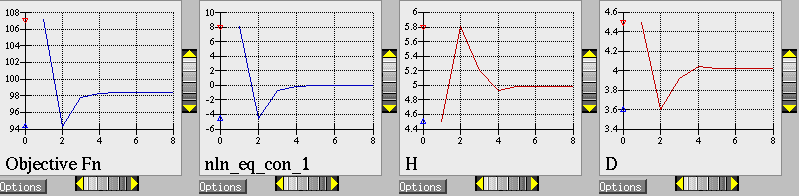
\includegraphics[width=\textwidth]{images/container_graphic}
\caption{Dakota 2D graphics for ``container'' problem showing history of
an objective function, an equality constraint, and two variables.}
\label{output:2dcont}
\end{figure}

The scroll bars which are located on each graph below and to the right
of each plot may be operated by dragging on the bars or pressing the
arrows, both of which result in expansion/contraction of the axis
scale. Clicking on the ``Options'' button results in the window shown
in Figure~\ref{output:2dcontoptions}, which allows the user to include
min/max markers on the vertical axis, vertical and horizontal axis
labels, and a plot legend within the corresponding graphics plot.  In
addition, the values of either or both axes may be plotted using a
logarithmic scale (so long as all plot values are greater than zero)
and an encapsulated postscript (EPS) file, named 
\texttt{dakota\_graphic\_\emph{i}.eps} where \emph{i} is the plot 
window number, can be created using the ``Print'' button.
\begin{figure}
\centering
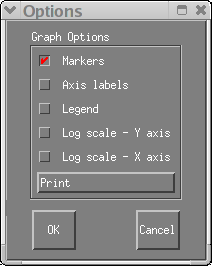
\includegraphics[scale=0.6]{images/container_graphic_options}
\caption{Options for Dakota 2D graphics.}
\label{output:2dcontoptions}
\end{figure}


\section{Error Messages Output}\label{output:error}

A variety of error messages are printed by Dakota in the event that an
error is detected in the input specification. Some of the more common
input errors, and the associated error messages, are described below.
See also the Common Specification Mistakes section in the Dakota
Reference Manual~\cite{RefMan}.

Incorrectly spelled specifications, such as 
\texttt{``numericl\_gradients''}, will result in error messages of the form:
\begin{small}
\begin{verbatim}
    Parser detected syntax error: unrecognized identifier 'numericl_gradients'
      within responses keyword.
    Please refer to the dakota.input.txt distributed with this executable.
\end{verbatim}
\end{small}

The input parser catches syntax errors, but not logic errors. The fact
that certain input combinations are erroneous must be detected after
parsing, at object construction time. For example, if a
\texttt{no\_gradients} specification for a response data set is
combined with selection of a gradient-based optimization method, then
this error must be detected during set-up of the optimizer (see last
line of listing):
\begin{small}
\begin{verbatim}
    Running MPI executable in serial mode.
    Dakota version 4.0 released 05/12/2006.
    Writing new restart file dakota.rst
    Constructing Single Method Strategy...
    methodName = npsol_sqp
    gradientType = none
    hessianType = none

    Error: gradient-based optimizers require a gradient specification.
\end{verbatim}
\end{small}

Another common mistake involves a mismatch between the amount of data
expected on a function evaluation and the data returned by the user's
simulation code or driver. The available response data is specified in
the responses keyword block, and the subset of this data needed for a
particular evaluation is managed by the active set vector. For
example, if Dakota expects function values and gradients to be
returned (as indicated by an active set vector containing 3's), but
the user's simulation code only returns function values, then the
following error message is generated:
\begin{small}
\begin{verbatim}
    At EOF: insufficient data for functionGradient 1
\end{verbatim}
\end{small}

Unfortunately, descriptive error messages are not available for all
possible failure modes of Dakota. If you encounter core dumps,
segmentation faults, or other failures, please request help using the
support mechanisms described on the
\href{http://dakota.sandia.gov/}{Dakota website}.

\section{Variables Output from Pre-run}

The pre-run mode (supported only for select methods) permits
specification of an output file to which Dakota will write parameter
(variables) data in annotated format (see
Section~\ref{input:tabularformat}) with data columns corresponding to
each variable.  This file can be generated with sampling, parameter
study, and DACE methods by invoking
\begin{small}
\begin{verbatim}
    dakota -i dakota.in -pre_run ::variables.dat
\end{verbatim}
\end{small}
for example, to output the variables (samples) in an LHS study.
